% Allow relative paths in included subfiles that are compiled separately
% See https://tex.stackexchange.com/questions/153312/
\providecommand{\main}{..}
\documentclass[\main/thesis.tex]{subfiles}
\onlyinsubfile{\zexternaldocument*{\main/tex/introduction}}

\begin{document}
\chapter{Drum-Kit Mutation}
\section{Suitability for Live Performance}

We originally set out to generate new drum samples for the purpose of creating new drum-kits which musicians could use to create drum tracks for their compositions. One use case for the drum generation approach pursued in this work is to create and evolve drum-kits on the fly.  In order to test the suitability of the generative system for both drum-kit generation and live performances, we designed a framework which utilizes the generative system to create a~\enquote{live performance} framework as outlined in Figure~\ref{fig:live_drumming}. This framework continually evolves the sounds within a drum-pattern (or rhythm) by creating and mutating a drum-kit using the outputs of the best TPE system. This framework could be particularly useful in a setting where drum rhythms are repeated for long durations. In order to test this approach, we created a basic music notation program where each drum track is defined by the following attributes:

\begin{itemize}
    \item Beats Per Minute (BPM): This defines the \enquote{speed} of the pattern. 
    \item Number of Beats: How many beats are in the pattern.
    \item Drum Pattern: An action must be taken at each beat, either a drum is played or no action is taken and nothing is played for that beat. The drum pattern dictates what action is taken at each beat. This makes the drum patterns monophonic (at most one sound can be played at a time).
\end{itemize}

\begin{figure}[tpb]
    \begin{center}
    \textbf{Drum Track Generation}
    \makebox[\textwidth]{
    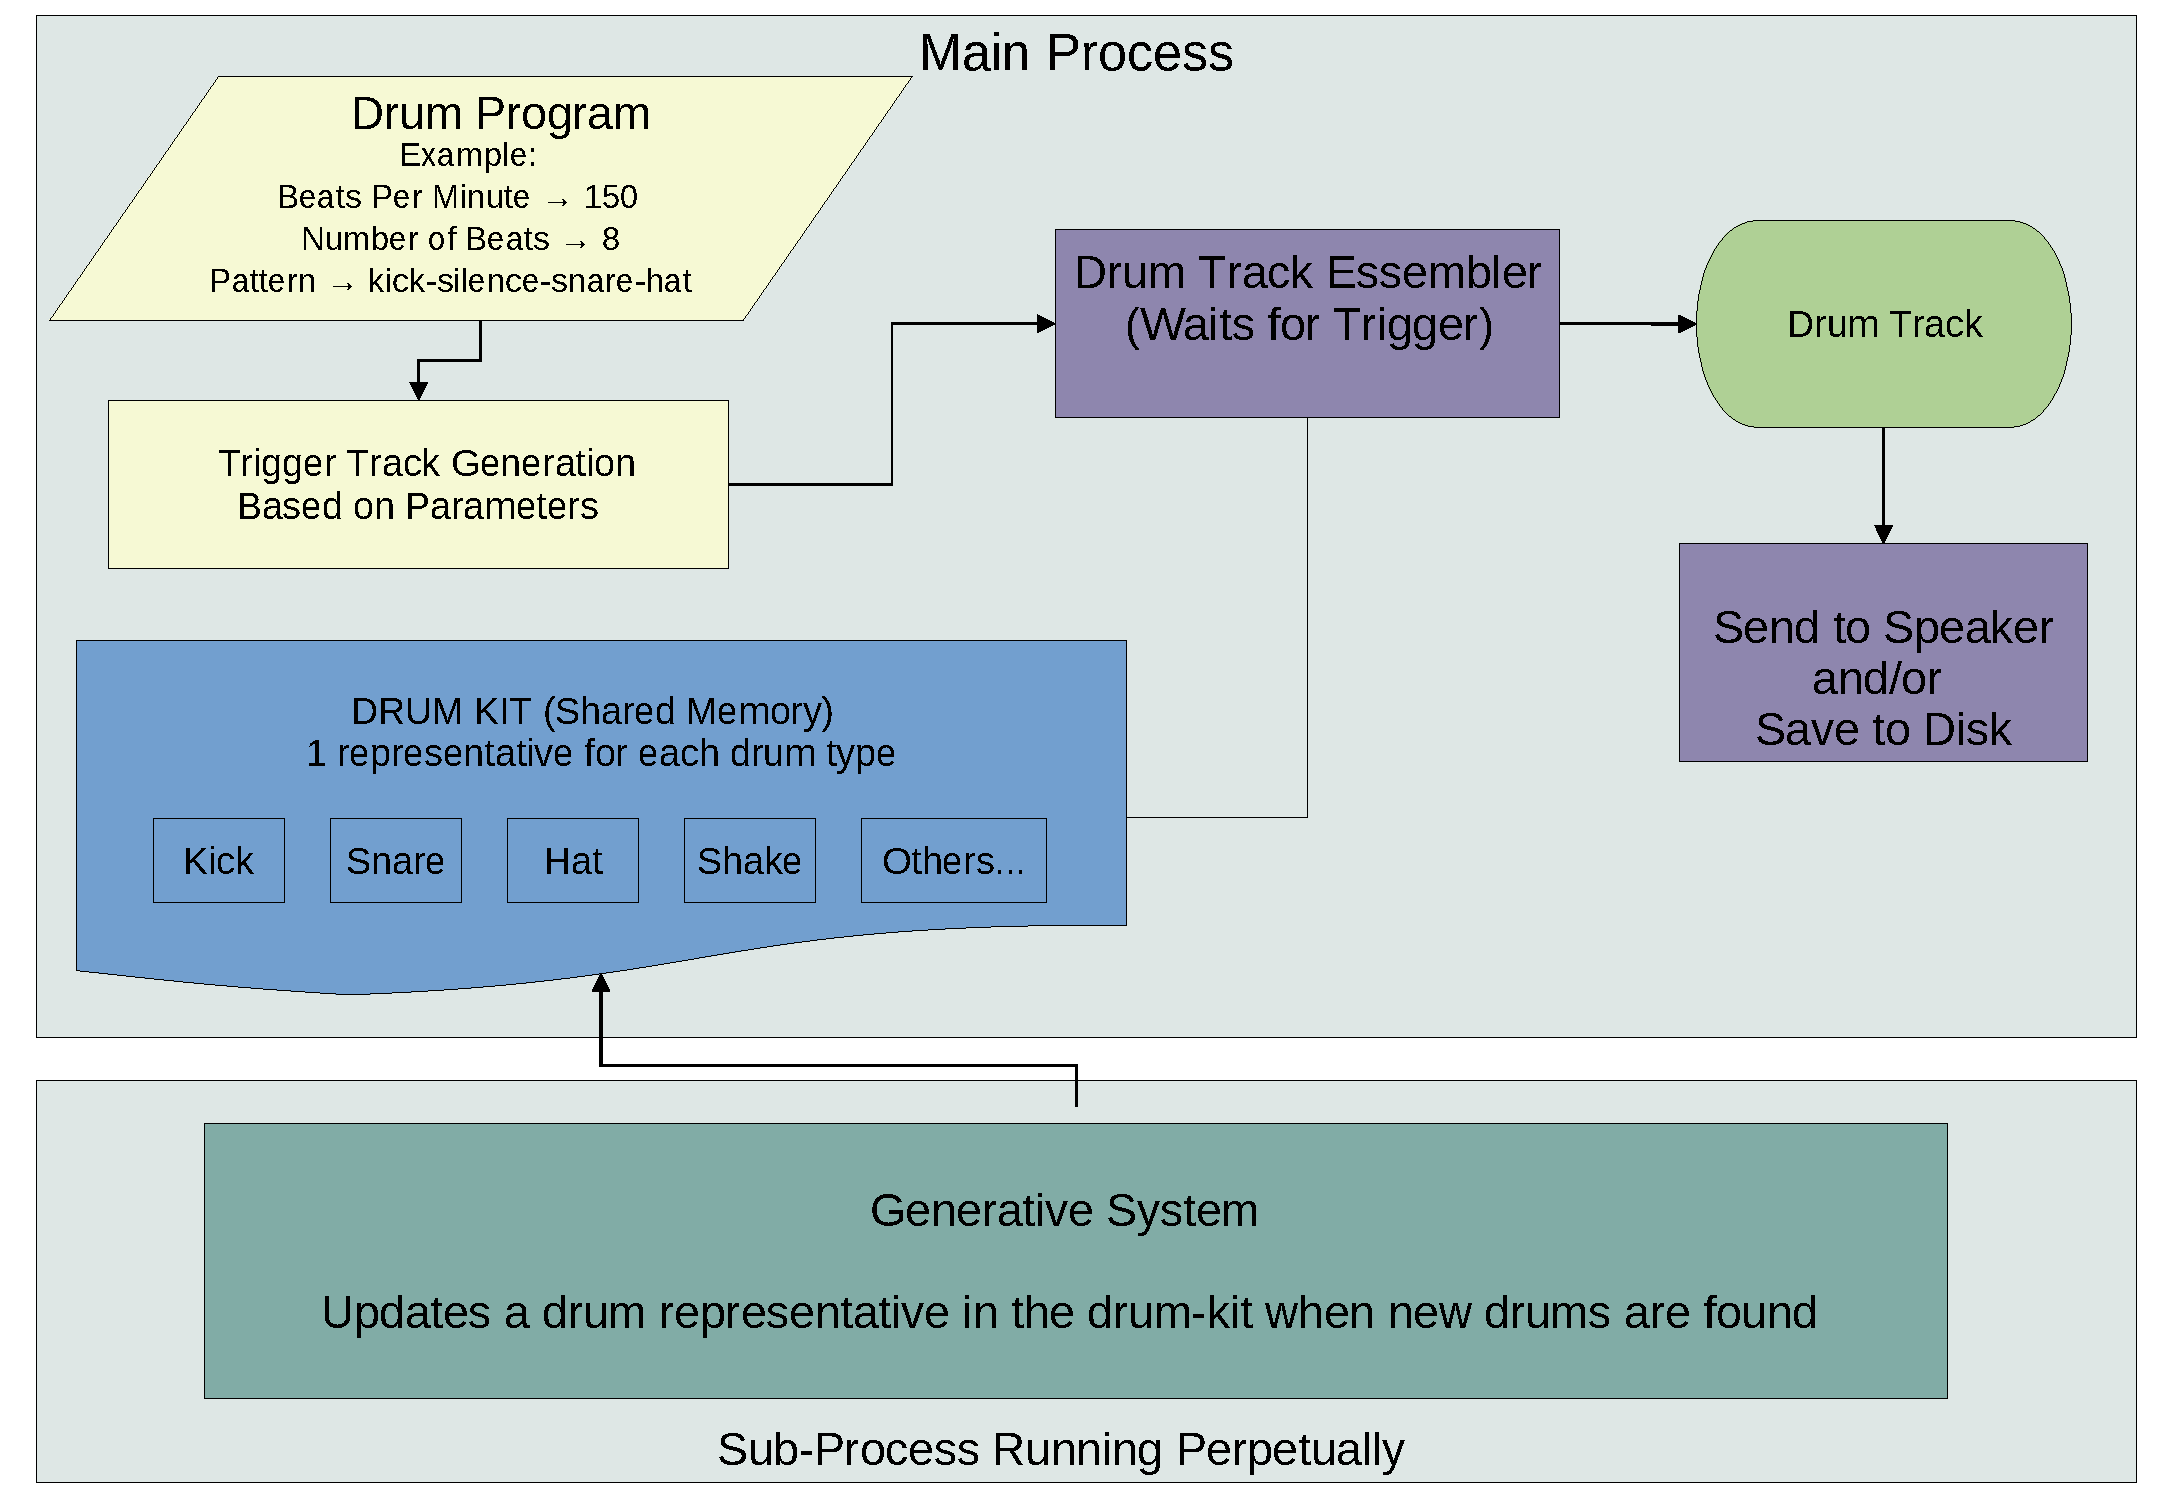
\includegraphics[width=1.1\linewidth]{images/live_programming.pdf}}
    \end{center}
    \caption{Live drum programming framework. Given a pre-defined drum program, the main process creates drum tracks using a drum-kit. This drum-kit is continually modified by a generative system running in a background process. In a live setting, the drum track assembler can be triggered at set times depending on the program, in offline generation, it can be triggered whenever there is a modification to the drum-kit.  }
\label{fig:live_drumming}
\end{figure} 

This experiment starts with a drum program and a drum-kit which contains 1 representative for the hat, kick, snare and shaker percussion categories. Next, a process begins to perpetually listen for new outputs from the TPE system. Each time a new drum sound is created, the process replaces a sound in the drum-kit depending on the drum category; next, the drum track is regenerated using the new drum-kit. With this approach, if the outputs are listened to sequentially or in a live setting, the same rhythm is repeated, but the drums within the rhythm mutate over time. To analyse this approach, we defined two simple drum programs (shown in Table~\ref{tab:drum_prog}), and let the experiment run until 1000 drum tracks are generated, that is, 1000 new drum sounds are found and used for the creation of a drum track. The results for the rendition of the programs are available for download on Zenodo\footnote{https://zenodo.org/record/5202776}. 
%     loop = add_to_loop(loop,"kick",0,drum_kit)
%     loop = add_to_loop(loop,"kick",2,drum_kit)
%     loop = add_to_loop(loop,"snare",4,drum_kit)
%     loop = add_to_loop(loop,"hat",6,drum_kit)
% #     loop = add_to_loop(loop,"shake",7,drum_kit)
%     loop = add_to_loop(loop,"hat",8,drum_kit)
%     loop = add_to_loop(loop,"shake",9,drum_kit)
%     loop = add_to_loop(loop,"kick",10,drum_kit)
%     loop = add_to_loop(loop,"snare",12,drum_kit)
\begin{table}[tbp]
 \resizebox{\linewidth}{!}{
     \begin{tabular}{|l|l|l|l|}
    \hline
    Program & BPM & Beats & Action at Each Beat \\ \hline
    
    Loop 1  & 180 & 8   & Kick-Snare-Hat-Kick-Snare-Hat-Kick-Shake     \\ \hline
    Loop 2  & 125 & 16   & Kick-.-Kick-.-Snare-.-Hat-Shake-Hat-Shake-Kick-.-Snare-.-.     \\ \hline
    % Loop 2  & 300 & 7               &   in progress &       \\ \hline
    \end{tabular}
 }
\caption{\label{tab:drum_prog} Parameters for each drum program. A period (\enquote{.}) indicates no action}
\end{table}
\section{Analyzing the Outputs}
 We conduct a listening test in order to quantify the usefulness of this framework. For this test, Amir Salimi and Abram Hindle listened to 100 drum tracks for each drum program and recorded the number of drum tracks they personally found appropriate for their live performance, that is, the rendered track accurately represented the underlying drum program. The result of this survey is shown in Table~\ref{tab:track_likes}. Due to the subjective nature of this analysis, readers are encouraged to download and analyze the results as well. We consider the majority of the drum tracks output by this system to be successful renditions. As discussed previously in Section~\ref{survey-conc}, as many as 30\% of the drum sounds output by the TPE system did not resemble drums when played in isolation. However, within a larger rhythmic pattern, the effect of these failures is diminished and can at times introduce an interesting dimension to the tracks. We also note that due the the source of drum sounds that are learned from and imitated in this work, generation of drum tracks may be more suitable for experimental music performances.
 
  We monitored the drum discovery rate while rendering the drum programs, and found that the relative ratio of drum to non-drum generations was approximately 1/100. This means that 100 sounds need to be created before 1 modification is made to the drum-kit. Using 1 CPU thread\footnote{AMD Ryzen 7 2700X Eight-Core Processor}, these 100 iterations take approximately 7 seconds. This discovery rate can be increased or decreased in a number of ways. For example, by increasing the number of discovery threads at the cost of heavier load to the CPU. It is also possible to make trade-offs in precision and sensitivity, that is, accepting more sounds that may not fit their role well within the composition and decreasing discovery time, or rejecting more unsuitable sounds and increasing discovery time. 
\begin{table}[tbp]
 \resizebox{\linewidth}{!}{
\begin{tabular}{|l|l|l|l|}
\hline
Program & Listener 1 Likes/100 & Listener 2 Likes/100 & Average Percentage \\ \hline
Loop 1  & 73/100                 & 54/100                   & 68\%               \\ \hline
Loop 1  & 55/100                 & 55/100                   & 55\%               \\ \hline
\end{tabular}       
 }
\caption{\label{tab:track_likes} Measuring the quality of generated drum tracks by calculating the percentage of liked outputs for each listener.}
\end{table}


\subsection{Noticeable Limitations}
 These drum tracks highlight other issues and limitations of this work. Other than improving the virtual ears, some of the issues and possible solutions are as follows:
~\begin{itemize}
    \item  Discovery time: Stricter,  more  powerful  drum  versus  non-drum  classifiers may reject nearly all synthesized outputs, making the creation of new drum-kits time consuming if not impossible. This means that the introduction of an algorithm which intelligently  modifies  parameters in order to successfully make drums will be a necessary step in the future in order to create desired sounds more efficiently.
    
    \item Limited variety: The virtual synthesizer used in this work has a limited set of parameters. This causes a lack of variety in the sounds output by the system. Expansion of the virtual synthesizer parameters or an interface which allows the use of VST synthesizers could help with this problem.
    
    % \item Cohesiveness: Drum-kits are typically put together manually such that little to no modifications are needed before improvisation or composition. Here the sounds are generated independently, therefore there can be loudness and harmonic discrepancies within the drum-kits. Normalization, filtering, and other DSP techniques can help with the creation of more cohesive kits. 
\end{itemize}
\section{Conclusion}
The goal here was to create a tool which can create and mutate drums used within drum-tracks for live performances. In an offline setting, this tool should be able to quickly generate new drum-kits for musicians. To this end, we implemented a simple framework which creates drum tracks given a drum pattern. 

This framework uses the generative system of drums described in the previous chapters to gradually replace the drum sounds within the drum pattern (i.e., the underlying drum-kit). We analyzed the outputs of this framework and believe that many of the outputs could be useful for musicians. 

 This experiment shows that the approach taken in this work towards a generative system of drum sounds can have many creative applications. While some of the weaknesses and failures of the classification models may be less pronounced in a live performance, this experiment also highlights other possible avenues of improvement and expansion which we hope to address in future works.

\end{document}


% \begin{table}[]
% \begin{center}

% \begin{tabular}{|l|l|l|}
% \hline
%       & Number of Replacements & Percent \\ \hline
% Kick   &                        &         \\ \hline
% Snare  &                        &         \\ \hline
% Hat    &                        &         \\ \hline
% Shaker &                        &         \\ \hline
% Total  &                        &         \\ \hline
% \end{tabular}
% \end{center}
% \end{table}